\documentclass[11pt,a4paper,ngerman]{article}
\usepackage[bottom=2.5cm,top=2.5cm]{geometry} 
\usepackage{babel}
\usepackage[utf8]{inputenc} 
\usepackage[T1]{fontenc} 
\usepackage{ae} 
\usepackage{amssymb} 
\usepackage{amsmath}
\usepackage{amsthm} 
\usepackage{graphicx}
\usepackage{fancyhdr}
\usepackage{fancyref}
\usepackage{listings}
\usepackage{xcolor}
\usepackage{paralist}

\usepackage[pdftex, bookmarks=false, pdfstartview={FitH}, linkbordercolor=white]{hyperref}
\usepackage{fancyhdr}
\pagestyle{fancy}
\fancyhead[C]{Computational Geometry}
\fancyhead[L]{Exercise sheet 2}
\fancyhead[R]{SoSe 2013}
\fancyfoot{}
\fancyfoot[L]{}
\fancyfoot[C]{\thepage \hspace{1px} of \pageref{LastPage}}
\renewcommand{\footrulewidth}{0.5pt}
\renewcommand{\headrulewidth}{0.5pt}
\setlength{\parindent}{0pt} 
\setlength{\headheight}{0pt}

\date{}
\title{Exercise sheet 2}
\author{Max Wisniewski, Alexander Steen}


%%
%% Enviroments for proofs and lemmas
%%
\newtheorem{lemma}{\bfseries Claim}

\begin{document}

\lstset{language=Pascal, basicstyle=\ttfamily\fontsize{10pt}{10pt}\selectfont\upshape, commentstyle=\rmfamily\slshape, keywordstyle=\rmfamily\bfseries, breaklines=true, frame=single, xleftmargin=3mm, xrightmargin=3mm, tabsize=2, mathescape=true}

\renewcommand{\figurename}{Figure}

\maketitle
\thispagestyle{fancy}

\begin{description}
%%%%%%%%%%%%%%%%%%%%%%%%
%% Aufgabe 1 
%%%%%%%%%%%%%%%%%%%%%%%%
\item[Problem 1] Convexity
  \begin{enumerate}[a)]
    \item Let $\{C_i\}_{i \in I}$ be a set of convex sets. Show that $\bigcap_{i \in I} C_i$ is convex.\\

          \textbf{Proof}: Since each $C_i$ is convex, it holds that the line $\overline{pq}$,
                          for $p,q \in C_i$, is completely contained in $C_i$. 
                          %%More formally
                          %%$\forall p,q \in C_i \, \forall \alpha \in [0,1]:
                          %%(1- \alpha) p + \alpha (q-p) \in C_i$, for all $i$. 
                          Since for all $p,q \in \bigcap_{i \in I} C_i$, the segment 
                          $\overline{pq}$ is contained in each $C_i$, it holds that
                          $\overline{pq} \in \bigcap_{i \in I} C_i$.\\
                          $\Rightarrow \bigcap_{i \in I} C_i$ is convex.
                          \mbox{} \hfill $\square$ \\

          A similar property can be found for unions of convex sets: \\        
          \textbf{Claim}: For any non-decreasing series of
                          convex sets $(C_i)_{i \in I}$ (with respect to set inclusion),
                          the set $\bigcup_{i \in I} C_i$ is convex.\\
          \textbf{Proof}: For all $p,q \in \bigcup_{i \in I} C_i$ there exists a $\tilde{i} \in I$
                          such that $p,q \in C_{\tilde{i}}$, hence $\overline{pq} \in C_{\tilde{i}}$.
                          Since $(C_i)_{i \in I}$ is non-decreasing,
                          $\overline{pq} \in \bigcup_{i \in I} C_i$.
                          \mbox{} \hfill $\square$ 
                          
    \item Let $P$ be a finite point set in the plane.
          Show that the boundary of the convex hull $CH(P)$ of $P$ is a convex polygon
          whose vertices are points of $P$. \\

     \textbf{Proof:}\\
     We first proove, that $CH(P)$ is a polygon and second, the 
     points of the polygon are points of $P$.\\

     Let $C$ be an arbitrary convex set containing $P$. Assume $C$ is
    not a polygon. Fix a point $x$ on that curve 
    \footnote{We assume complete sets. If the set has no boundary
    we consider a series of points converging to the boundary.}.
    We now take $\varepsilon > 0$ steps on the curve to the point
    $x_\varepsilon$ and look at the 
    set $C'$ where we substituted the line $\overline{xx_\varepsilon}$
    for the curveseqment that connected them before.

    We know if $\varepsilon$ is small enough there is no point of $P$
    in the cut part. If the curve was bend left, the resulting line will
    only do left turns at the end. Therefore $C'$ is convex.

    Hence $C$ could not be the convex hull.\\

    Next we fix a convex polygon $CP$ that has points of $P$ on the
    nodes. This can be found by intersecting all halfplanes that contain all
    points in $P$ as in the Brute-Force algorithm.\\

    Because $CP$ is a convex set containing $P$ only 
    $CH(P) \subset CP$ can hold.\\

    Assume there is a point on the polygon $CH(P)$ $y=p_k \not \in P$.
    Then $p_{k-1}p_kp_{k+1}$ is a triangle pointing to the outside
    of the polygon. Otherwise we would have taken a left turn in cw
    order.
    But this is not possible due to the previous shown fact, that
    a polygon only of points of $P$ is a convex set containing $P$.
    Hence $p_k$ can not be on the hull.\\
\mbox{}\hfill$\square$

    \item Show that the segment between two points $p, q \in P$ is an edge of $CH(P)$ if
          and only if all points of $P$ lie on the same side of the line through $p$ and $q$. \\

          \textbf{Proof}: \\
          "$\Rightarrow$": By contraposition. Let $\tilde{p}$ a point on the one side of the line
                           through $p$ and $q$ and $\tilde{q}$ a point on the other side.
                           Let $s \in \overline{pq}$. Then, one of $\overline{s\tilde{p}}$ 
                           and $\overline{s\tilde{q}}$ is not contained in $P$. Hence,
                           $\overline{pq}$ cannot be an edge of $CH(P)$. \\
          "$\Leftarrow$": \\
        By the previous part, we know that the $CH(P)$ is a polygon
        of the points in $P$. Because $p,q \in P$ we know that 
        $\overline{pq} \in CH(P)$.\\ 

        Assume $\overline{pq}$ is not
        on the boundary. Then there exists points $u,v \in P$
        on both sides of $\overline{pq}$ by the previous part.
        But this is not possible due to the premise.
                
          \mbox{} \hfill $\square$
  \end{enumerate}

%%%%%%%%%%%%%%%%%%%%%%%%
%% Aufgabe 2
%%%%%%%%%%%%%%%%%%%%%%%%
\item[Problem 2] Computing the maximal tangent to a subconvex hull in Chens Algorithm in $O(log h^*)$. \\

\textbf{Proof:}\\

Let $p_{k-1}, p_k$ be the last computed points on the convex hull.
Let $q_1, ..., q_{h^*}$ be the points on the convex hull of the subconvex hull
given in ccw or cw order. Then we will compute the point on the hull that
maximizes the angle as follows. Assume we have the points given in an array
\lstinline|hull|.

\begin{lstlisting}[mathescape=true]
pos $\leftarrow$ 1
h'$\leftarrow h^*$ / 2
while h' > 0 do
  l $\leftarrow$ deg($p_{k-1},p_k$,hull[pos-1 mod h^*]))
  c $\leftarrow$ deg($p_{k-1},p_k$,hull[pos mod h^*]))
  r $\leftarrow$ deg($p_{k-1},p_k$,hull[pos+1 mod h^*]))
  if l < c && c < r || l == r
    pos $\leftarrow$ pos + h' mod $h^*$
  else if l > c && c > r
    pos $\leftarrow$ pos - h' mod $h^*$
  h'$\leftarrow$ h' / 2
od
return pos
\end{lstlisting}

Next we have to verify the algorithm.
\begin{lemma}\label{alge:ueb2:logh}
  The above algorithm maximizes the angle and can be
  computed in $O(\log \, h^*)$ time.\\
\mbox{}\hfill$\lrcorner$
\end{lemma}

\textbf{Proof \ref{alge:ueb2:logh}:}\\
The running time of the algorithm is obviously $O(\log \, h^*)$.
We start with $\frac{h^*}{2}$. In the while loop we only
compute for constant time $c$. We decrease $h'$ until we hit zero.
$$
\Rightarrow T(n) = log h^*.
$$

We know that $\overset{\infty}{\underset{i=1}{\sum \frac{h^*}{2}}} = h^*$
and if our steps are discrete we can reach the point in $log h^*$ time
(Binary Search).
Let $R_i$ be the set of reachable points on the hull in step $i$
of the algorithm and $q$ the optimal point. Then
$$
    \forall i \in \mathbb{N} : q \in R_i, |R_i| = \frac{h^*}{2^i}
$$
Inducion on $i$.
\begin{description}
    \item[\bfseries I.A.] $i=1$\\
    In the first step we can do at most 
    $\overset{\infty}{\underset{i=1}{\sum}} \frac{h^*}{2^i} = h^*$
    steps. Therefore all points are reachable espacially $q$.
    \item[\bfseries I.S.] $i \leadsto i+1$\\
    We now in $q \in R_i$. On the last step we were
    according to the algorithm at one endpoint and we were on the
    edge of $R_i$. In the algorithm we devide \lstinline|h'| by two,
    therefore we are in the middle of the set according to the given order
    because it had size \lstinline|h'| $= |R_i|$.
    We divide $R_i$ into two subsets $R_{i+1}^l$ and $R_{i+1}^r$.
    If the first case is true, we know $q \in R_{i+1}^l$ because
    the hull was convex therefore we can only decrease the angle again
    on the otherside of the optimum. We take $R_{i+1}=R_{i+1}^l$
    as the algorithm says. The othercase is equivalent with $R_{i+1}^r$.\\
    $|R_{i+1}| = |\frac{R_i}{2}|$.
\end{description}
BUILD UP MORE!!
\mbox{}\hfill$\square$



%%%%%%%%%%%%%%%%%%%%%%%%
%% Aufgabe 3
%%%%%%%%%%%%%%%%%%%%%%%%
\item[Problem 3] Chan's algorithm and superexponential search
  \begin{enumerate}[a)]
    \item Show that the first $h^*$ points of the convex hull
        can be computed in $O(n)$ time given the $r$ subconvex hulls.\\
    \textbf{Solution:}\\
        Given an two dimensional array \lstinline|hulls| where
        \lstinline|hull[i]| is the array of points of the $i$-th hull
        and \lstinline|hull[i][j]| is the $j$-th point of the $i$-th hull
        in ccw order.\\
        Let $p_0, p_1$ be the first points as given in the algorithm. 
        The array \lstinline|act| contains for each hull the index
        of the point that maximizes the angle in the current step. Then
        we compute the algorithm as follows.
\begin{lstlisting}[mathescape=true]
int[n] act
compute act[i] with algorithm in ex. 2
for k = 2 to $h^*$ - 1 
    for i = 1 to n / $h^*$
        while angle($p_{k-1}$, $p_k$, hull[i][act[i]]) < angle(($p_{k-1}$, $p_k$, hull[i][act[i+1 mod $h^*$]])
            act[i] = (act[i] + 1) mod $h^*$
    i'=$\underset{0 \leq i < h^* / n}{\text{argmax}}$ angle(($p_{k-1}$, $p_k$, hull[i][act[i+1 mod $h^*$]]
    $p_{k+1}$ = hull[i'][act[i']]
\end{lstlisting}

    After the initial searching of the max we will just proceed in the ccw order of the
    hull.
    \begin{lemma}\label{alge:ueb2:p3}
        The above algorithm computes the first $h^*$ points of the convex hull
        and runs in $O(n)$ time.\\
        \mbox{}\hfill$\lrcorner$
    \end{lemma}

    \textbf{Proof \ref{alge:ueb2:p3}.}
        Given the correctness of chan's algorithm we only changed the computation
        of the next maximum angle in each step. We do not do a binary search
        in each step, but go through the list linear. In this iteration we
        will find of course the maximum angle, due to the termination criterion of
        the while loop. This maximum exists and will therefor be found.\\

        Next we show, that each point on the small convex hulls will only be
        considered twice through all iterations.\\

        Let $0 \leq i < n / h^*$ be arbitrary but fixed the $i$-th hull and
        $1 \leq x \leq h^*$ be the index of the $x$-point of the $i$-th hull.\\

        If we started with \lstinline|hull[i][x]| it is on the hull. Therefor
        if we get the index again we will eventually after finite steps
        take this point into the hull. Hence we consider $x$ to be a maximal
        point in round $k > 1$. Let $p_{k-1}, p_k$ the last computed points
        on the hull.
        If we look at the picture in figure \ref{alge:ueb2:hullOn}
        if we assume the convex polygon has a border after $x$ at most 
        at the line $\overline{p_kx}$ and assumed somewhere on the corssing line.
        The next point from which $x$ is no longer the maximizing point is
        element of $P_1$ potentially $x$ itself.\\
        If we want to leave $x$ behind us a second time we have to cross $p_{k-1}$
        again. But to come by $p_{k-1}$ we have to be up left in $P_2$ with some
        point $p_{k+t}$ such that it is convex. But there is no way we can
        cross $p_{k-1}$\footnote{By crossing we mean passing the line given
        by the normal on $\overline{p_{k-1}p_k}$ and and the point $p_{k-1}$ itself.}
        We can either connect to $p_{k-1}$ such that the polygon is closed in the
        algorithm finishes. Or we come above or below $p_{k-1}$.
        This is not possible because all lines of the algorithm are borders
        of the polygon. Now either $\overline{p_{k+t}p_{k+t+1}}$ is on the left
        of $\overline{p_{k-1}p_k}$ in which case $\overline{p_{k+t}p_{k+t+1}}$ is
        no borderline or it is the otherway around.\\

        We conclude, that it is not possible to enter $P_1$ a second time,
        such that we will consider $x$ only twice.\\

        This shows us, that the innermost loop can only skip each element once.
        \begin{figure}[tb]
            \centering
            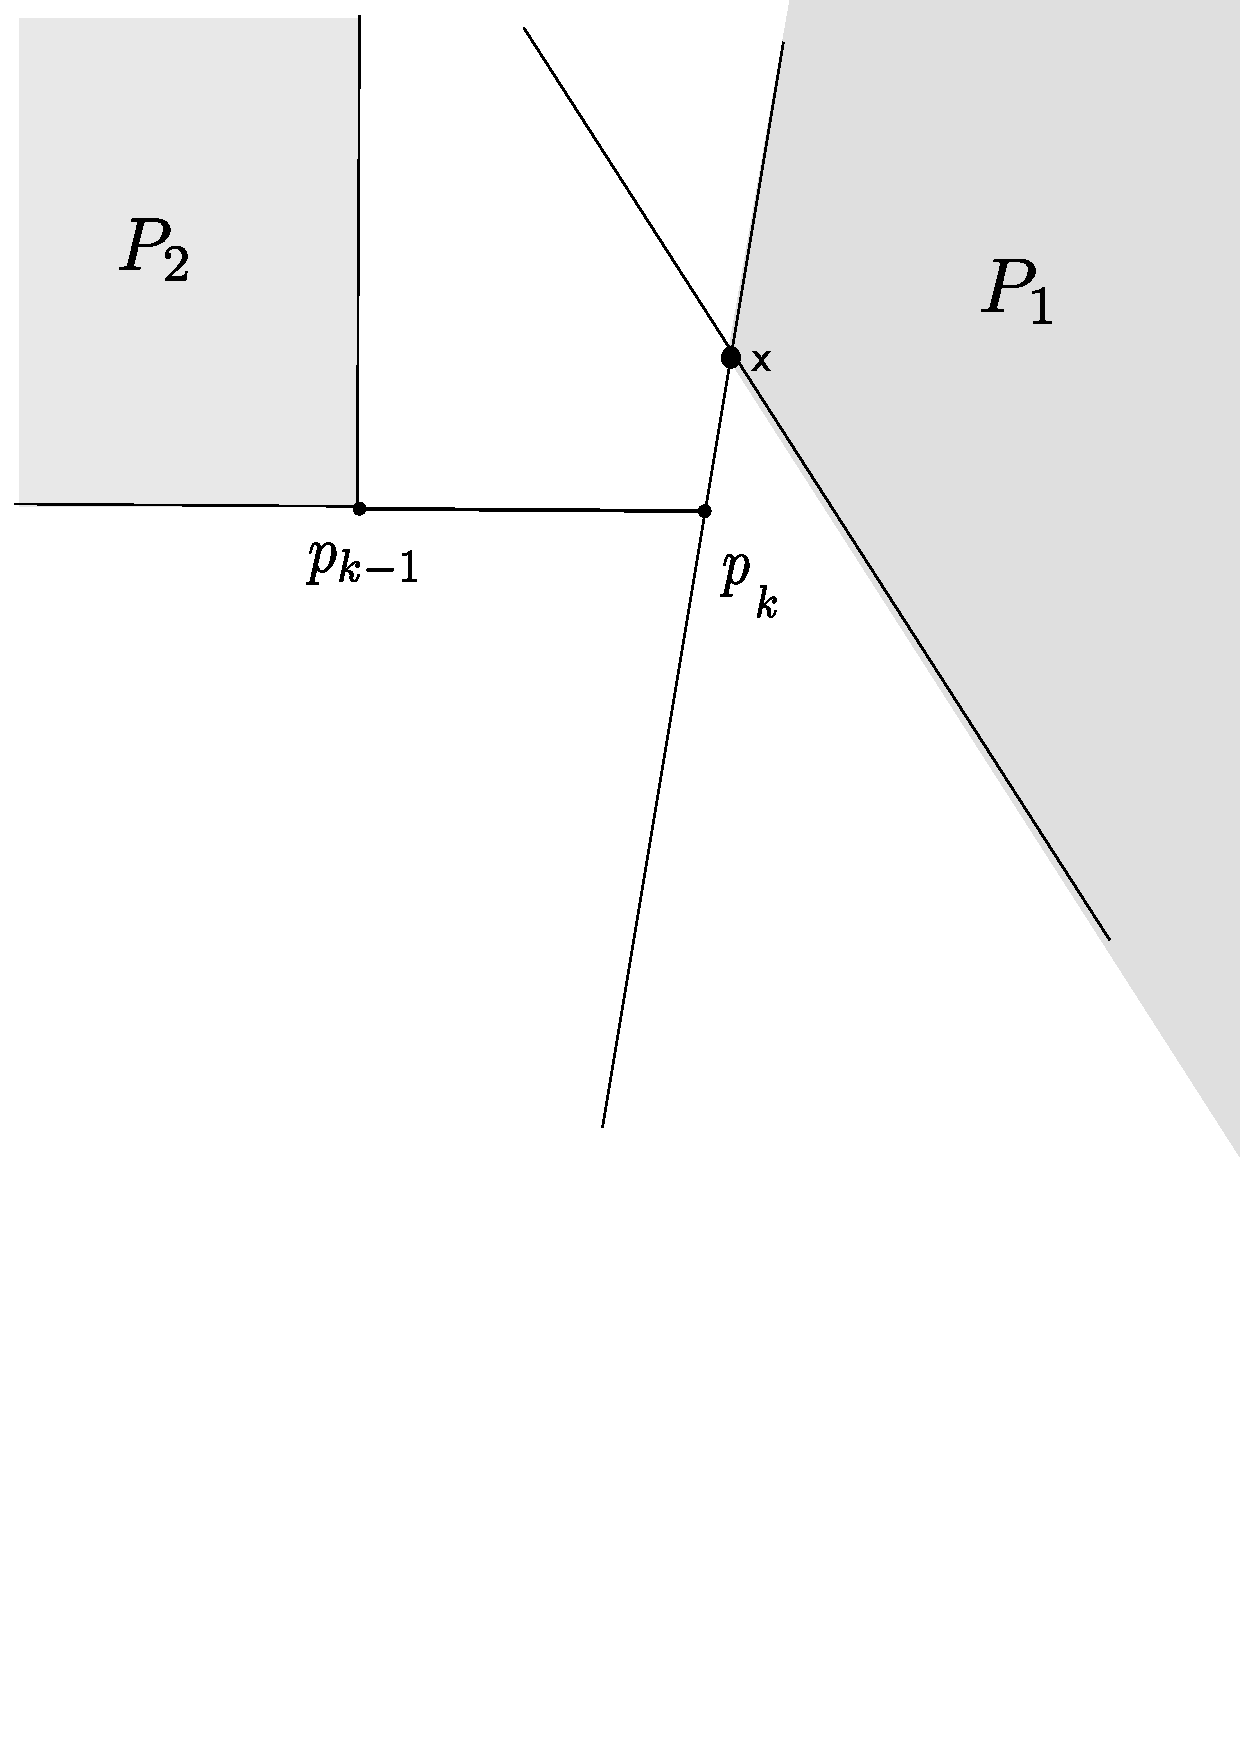
\includegraphics[clip, trim = 0mm 14cm 5mm 7mm, width = 0.8\textwidth]{pictures/itHull}
            \caption{Spaces able to consider $x$ as a point.}
            \label{alge:ueb2:hullOn}
        \end{figure}

        The running time consists of
        \begin{enumerate}[1)]
            \item Computing the $n / h^*$ starting points on the hulls.
                For each hull we can compute the point in $O(\log h^*)$.\\
                $\Rightarrow O(n)$ total running time.
            \item The internal for and while loops consider all points at most
                twice as prooven above. This gives a runtime of $O(n)$ in total.
            \item The maximum can be found in $O(n / h^*)$ and we compute it $h^*$
                times. The running time therefor is $O(n)$ in total.
        \end{enumerate}
        The algorithm has a runningtime of $T(n) = 3 \cdot O(n) = O(n)$.
        \mbox{}\hfill$\square$ 

    \item Show that by $2^{2^i}$ as the iteration for $h^*$ we obtain
        a total running time of $O(n \log h)$.\\
    \textbf{Proof:}\\
        From the lecture we know, that the runningtime for
        one iteration of the algorithm with $h^*$ has the running time
        $O(n \log h^*)$.
        Iteration our $h^*$ gives us that 
        $$
            h^*_{i+1} = 2^{2^{i+1}} = \left( 2^{2^i}\right)^2 = \left( h^*_i \right)^2
        $$
        hence if we terminate in step $n$ it holds that $h^*_n \leq h^2$. Or
        we should have terminated bevore.\\
        \begin{equation}
            h^*_n = 2^{2^n} \leq h^2 \Rightarrow n \leq (\log \log h) + 1
        \end{equation}
        Therefor the total runningtime of all iterations is
        \begin{equation}
        \begin{aligned}
            T(n, h) &=& \overset{\log \log h + 1}{\underset{n = 1}{\sum}} n \log h^*_n
            = n \overset{\log \log h + 1}{\underset{n=1}{\sum}} \log h^*_n\\
            &=& n \overset{\log \log h + 1}{\underset{n=1}{\sum}} \log 2^{2^n}
            = n \overset{\log \log h + 1}{\underset{n=1}{\sum}} 2^n\\
            &=& n \frac{2^{\log \log h + 2} - 1}{2 - 1}\\
            &=& 4 \cdot n \cdot 2^{\log \log h}
            = 4 n \log h\\
            &=& O (n \log h)
        \end{aligned}
        \end{equation}
    \mbox{}\hfill$\square$
  \end{enumerate}

\end{description}

\label{LastPage}

\end{document}
